\section{Some useful results}

\begin{lemma}\label{graphIsString}
  Let $\Gamma$ be a transitive sggi over $n$ points such that the permutation representation graph have exactly $n-1$ edges. Then the graph of $\Gamma$ is a string.
\end{lemma}

\begin{proof}
  $\Gamma$ is transitive so its permutation representation graph is connected. Therefore, because there are $n-1$ edges for $n$ vertices, the graph must be a tree.

  \paragraph{}
  Suppose now, that there is a vertex with at least three incident edges. These edges must be labelled with three differents numbers, $i, j, k$ that describe three different involutions, $\rho_i, \rho_j$ and $\rho_k$. But at least two of these involutions are not adjacent and so must commute. It will be considered that the involution $\rho_i$ and $\rho_k$ does commute.

  \paragraph{}
  And so by proposition 3.5 of~\cite{cprGraph}, the permutation representation graph where only edges labelled with $i$ and $k$ are kept must only contains those patterns:
  \begin{itemize}
    \item Fixed points
    \item Isolated edge (labelled with $i$ or $k$)
    \item Double edge
    \item Alternating square
  \end{itemize}
  But in our case, there are already two edges labelled $i$ and $k$ that connect the same point to two differents points. So the only way it can be extended to a good pattern is with an alternating square. But the graph cannot have an alternating square because it is a tree and thus does not contains any cycle.

  \paragraph{}
  Thus no vertex can have three edges but the graph must be connected, so the only solution is a string.
\end{proof}

\begin{lemma}\label{rho0atEnd}
  Let $\Gamma$ be a sggi with generators $\rho_0, \rho_1 \dots$ such that its permutation representation graph is a string. If $\rho_0$ and $\rho_1$ are 2-transpositions, then an edge of $\rho_0$ must be placed at an end of the permutation representation graph.
\end{lemma}

\begin{proof}
  The permutation representation graph is a string so it cannot have alterning square or double edge, thus two involutions that must commute can not share a vertex. By definition of a sggi, the $\rho_0$ involution must commute with all other involutions except $\rho_1$.

  \paragraph{}
  The $\rho_0$ edges must only share vertices with $\rho_1$ but there are two edges for each involution. But each $\rho_0$ edge must be surrounded by two $\rho_1$ if it is not at an end of the graph. One $\rho_1$ edge can be spared if it is surrounded by two $\rho_0$ edges but even with that three $\rho_1$ edges are needed with a $\rho_0$ cannot be placed at an end of the graph but there are only have two of them. Therefore one $\rho_0$ edge is at an end of the graph.
\end{proof}

\begin{lemma}
  Let $\Gamma$ be a sggi generating $A_{11}$. Then $\Gamma$ contains at least two 4-transpositions if it is of rank 4 and at least one 4-transposition if its rank is 5.
\end{lemma}

\begin{proof}
  Suppose that there exists a sggi of rank 5 with only 2-transposition or a sggi of rank 4 with only one 4-transposition. In both case, there is exactly 10 edges for 11 vertices. Lemma~\ref{graphIsString} can be applied and thus the permutation representation graph of $\Gamma$ is a string.

  \paragraph{Rank 5}
  In this case, there are five involutions and all of them are 2-transpositions. Thus, by Lemma~\ref{rho0atEnd}, a $\rho_0$ edge must be at one end of the graph. By duality, the same can be done with $\rho_4$ and so there is a $\rho_4$ edge at the other end.

  \paragraph{}
  Because the other end is occupied, the other edge of $\rho_0$ cannot go there. So a $\rho_1$ edge must be between the two $\rho_0$ edge (see the proof of Lemma~\ref{rho0atEnd} for details). The same reasonning can be applied to $\rho_3$ by duality. At this point, the graph is the following:

  \begin{figure}[H]
    \begin{center}
      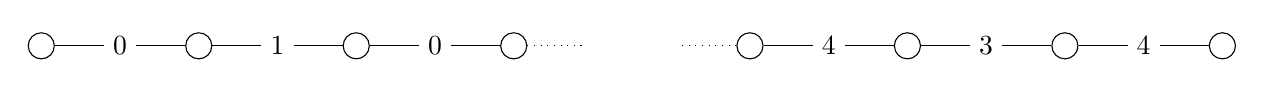
\begin{tikzpicture}

        \begin{scope}[every node/.style={circle,draw}]
          \node (1)  at (0,0)  {};
          \node (2)  at (2,0)  {};
          \node (3)  at (4,0)  {};
          \node (4)  at (6,0)  {};
          \node (8)  at (9,0)  {};
          \node (9)  at (11,0) {};
          \node (10) at (13,0) {};
          \node (11) at (15,0) {};
        \end{scope}

        \node (4b) at (7,0) {};
        \node (8b) at (8,0) {};

        \begin{scope}[every node/.style={fill=white}]
          \begin{scope}[every edge/.style={draw}]
            \path (1)  edge node {$0$} (2);
            \path (2)  edge node {$1$} (3);
            \path (3)  edge node {$0$} (4);
            \path (4)  edge[style={dotted}] (4b);
            \path (8)  edge[style={dotted}] (8b);
            \path (8)  edge node {$4$} (9);
            \path (9)  edge node {$3$} (10);
            \path (10) edge node {$4$} (11);
          \end{scope}
        \end{scope}



      \end{tikzpicture}
      \caption{}
    \end{center}
  \end{figure}

  \paragraph{}
  The $\rho_0$ and $\rho_4$ edges must be connected to something but the only possibility is to use a $\rho_1$ and a $\rho_3$ edge. Now the graph is the following and two $\rho_2$ edges must still be added to it. But they will be adjacent to each other and that is forbidden in a permutation representation graph.

  \begin{figure}[H]
    \begin{center}
      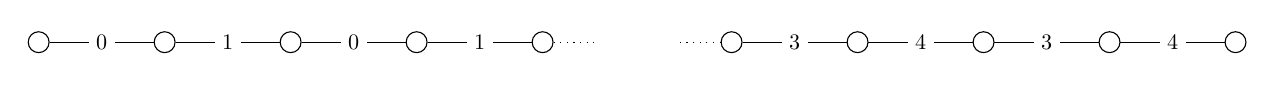
\begin{tikzpicture}[scale=0.8]

        \begin{scope}[every node/.style={circle,draw,transform shape}]
          \node (1)  at (0,0)  {};
          \node (2)  at (2,0)  {};
          \node (3)  at (4,0)  {};
          \node (4)  at (6,0)  {};
          \node (5)  at (8,0)  {};
          \node (7)  at (11,0) {};
          \node (8)  at (13,0) {};
          \node (9)  at (15,0) {};
          \node (10) at (17,0) {};
          \node (11) at (19,0) {};
        \end{scope}

        \node (5b) at (9,0) {};
        \node (7b) at (10,0) {};

        \begin{scope}[every node/.style={fill=white,transform shape}]

          \begin{scope}[every edge/.style={draw}]
            \path (1)  edge node {$0$} (2);
            \path (2)  edge node {$1$} (3);
            \path (3)  edge node {$0$} (4);
            \path (4)  edge node {$1$} (5);
            \path (5)  edge[style={dotted}] (5b);
            \path (7)  edge[style={dotted}] (7b);
            \path (7)  edge node {$3$} (8);
            \path (8)  edge node {$4$} (9);
            \path (9)  edge node {$3$} (10);
            \path (10) edge node {$4$} (11);
          \end{scope}
        \end{scope}



      \end{tikzpicture}
      \caption{}
    \end{center}
  \end{figure}


  \paragraph{Rank 4}
  There is exactly one 4-transposition. Thus, by duality, there are two cases: either $\rho_0$ or $\rho_1$ is a 4-transposition. If $\rho_0$ is a 4-transposition, then $\rho_1$ is a 2-transposition but all $\rho_0$ must be surrounded by $\rho_1$ involutions which is impossible.

  \paragraph{}
  So $\rho_1$ must be a 4-transposition. Therefore $\rho_2$ and $\rho_3$ are 2-transposition. And so by lemma~\ref{rho0atEnd}, a $\rho_3$ edge must be placed at an end, followed by a $\rho_2$ edge. For the other $\rho_3$ edge, there are two possibilities, it can be placed next to the first one or at the other end.

  \paragraph{}
  In the first case, the graph is the following. But the only way it can be completed is by using a sequence $\rho_1, \rho_0, \rho_1, \rho_0, \rho_1$ but there is still a $\rho_1$ edge that cannot be placed.

  \begin{figure}[H]
    \begin{center}
      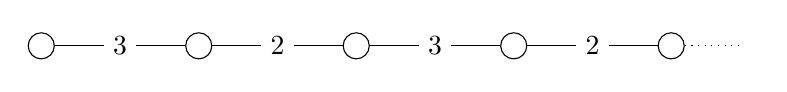
\begin{tikzpicture}

        \begin{scope}[every node/.style={circle,draw}]
          \node (1)  at (0,0)  {};
          \node (2)  at (2,0)  {};
          \node (3)  at (4,0)  {};
          \node (4)  at (6,0)  {};
          \node (5)  at (8,0)  {};
        \end{scope}

        \node (6)  at (9,0) {};

        \begin{scope}[every node/.style={fill=white}]

          \begin{scope}[every edge/.style={draw}]
            \path (1)  edge node {$3$} (2);
            \path (2)  edge node {$2$} (3);
            \path (3)  edge node {$3$} (4);
            \path (4)  edge node {$2$} (5);
            \path (5)  edge[style={dotted}] (6);
          \end{scope}
        \end{scope}

      \end{tikzpicture}
      \caption{}
    \end{center}
  \end{figure}

\paragraph{}
For the second case, that is the graph. On each side, it must be continued with a sequence $\rho_1, \rho_0, \rho_1$. And every edge is used but the middle point is linked with two $\rho_1$ edges and that is forbidden.

\begin{figure}[H]
  \begin{center}
    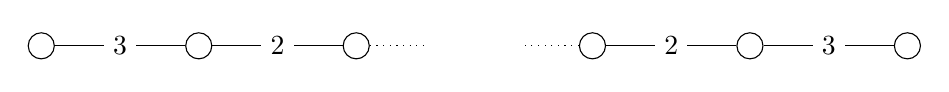
\begin{tikzpicture}

      \begin{scope}[every node/.style={circle,draw}]
        \node (1)  at (0,0)  {};
        \node (2)  at (2,0)  {};
        \node (3)  at (4,0)  {};
        \node (9)  at (7,0)  {};
        \node (10) at (9,0)  {};
        \node (11) at (11,0) {};
      \end{scope}

      \node (3b) at (5,0)  {};
      \node (9b) at (6,0)  {};


      \begin{scope}[every node/.style={fill=white}]

        \begin{scope}[every edge/.style={draw}]
          \path (1)  edge node {$3$} (2);
          \path (2)  edge node {$2$} (3);
          \path (3)  edge[style={dotted}] (3b);
          \path (9)  edge[style={dotted}] (9b);
          \path (9)  edge node {$2$} (10);
          \path (10) edge node {$3$} (11);
        \end{scope}
      \end{scope}

    \end{tikzpicture}
    \caption{}
  \end{center}
\end{figure}

\end{proof}
